\documentclass{beamer}

%% \documentclass[handout]{beamer}
%% % use this with the [handout] option to create handouts for the audience
%% \usepackage{pgfpages}
%% \pgfpagesuselayout{2 on 1}[a4paper,border shrink=5mm]

\mode<presentation>
{
  \usetheme{Diku}
% set this to your preferences:
  \setbeamercovered{invisible}
%  \setbeamercovered{transparent}
}

%\usepackage{listings}
%\usepackage{framed}
%\usepackage{graphicx}
%\usepackage{adjustbox}
%\usepackage{epic}
%\usepackage{url}
%\usepackage{paratype}
%\usepackage{xcolor}
%\usepackage{ulem}
%\usepackage{multirow}
%\setbeamerfont{frametitle}{family=\bf}
%
%\usepackage{amsmath}
%\usepackage{amssymb}
%\usepackage{amsthm}




\usepackage{listings}
\usepackage{graphicx}
\usepackage{epic}

\usepackage{amsmath}
\usepackage{amssymb}
\usepackage{amsthm}

\newcommand{\basetop}[1]{\vtop{\vskip-1ex\hbox{#1}}}
\newcommand{\source}[1]{\let\thefootnote\relax\footnotetext{\scriptsize\textcolor{kugray1}{Source: #1}}}

\lstdefinelanguage{Futhark}
{keywords={fun,if,then,else,loop,do,map,reduce,filter,scan,redomap,scatter,transpose,reshape,iota,replicate,let,in,for,while,with,i32,f32,int,zip,streamRed,zipWith, unsafe},%
  sensitive=true,%
  comment=[l]{--},%
  string=[b]",%
  moredelim=**[is][\color{red}]{@}{@},
  moredelim=**[is][\color{blue}]{¤}{¤},
}

\lstset{
  language=Futhark,
  basicstyle=\footnotesize
}


% for coloured code citation in text:
\usepackage{fancyvrb}

%%%%%%%%%%%%%%%%%%%%%%%%%%%%%%%%%
%%%%%    code sections   %%%%%%%%
%%%%%%%%%%%%%%%%%%%%%%%%%%%%%%%%%

% code highlighting commands in own block
\DefineVerbatimEnvironment{code}{Verbatim}{fontsize=\scriptsize}
\DefineVerbatimEnvironment{icode}{Verbatim}{fontsize=\scriptsize}

% Fancy code with color commands:
\DefineVerbatimEnvironment{colorcode}%
        {Verbatim}{fontsize=\scriptsize,commandchars=\\\{\}}

%%%%%%%%%%%%%%%%%%%%%%%%%%%%%%%%%%
%%%%%    some coloring    %%%%%%%%

%% use "DIKU green" from our color theme for \emph
%\renewcommand{\emph}[1]{\textcolor{structure}{#1}}
%% use some not-too-bright red for an \emp command
%\definecolor{DikuRed}{RGB}{130,50,32}
%\newcommand{\emp}[1]{\textcolor{DikuRed}{ #1}}
%\definecolor{CosGreen}{RGB}{10,100,70}
%\newcommand{\emphh}[1]{\textcolor{CosGreen}{ #1}}


\definecolor{Red}{RGB}{220,50,10}
\definecolor{Blue}{RGB}{0,51,102}
\definecolor{Yellow}{RGB}{102,51,0}
\definecolor{Orange}{RGB}{178,36,36}
\definecolor{Grey}{RGB}{180,180,180}
\definecolor{Green}{RGB}{20,120,20}
\definecolor{Purple}{RGB}{160,50,100}
\newcommand{\red}[1]{\textcolor{Red}{{#1}}}
\newcommand{\blue}[1]{\textcolor{Blue}{{#1}}}
\newcommand{\yellow}[1]{\textcolor{Yellow}{{#1}}}
\newcommand{\orange}[1]{\textcolor{Orange}{{#1}}}
\newcommand{\grey}[1]{\textcolor{Grey}{{#1}}}
\newcommand{\green}[1]{\textcolor{Green}{{#1}}}
\newcommand{\purple}[1]{\textcolor{Purple}{{#1}}}




% use "DIKU green" from our color theme for \emph
\renewcommand{\emph}[1]{\textcolor{structure}{#1}}
% use some not-too-bright red for an \emp command
\definecolor{DikuRed}{RGB}{130,50,32}
\newcommand{\emp}[1]{\textcolor{DikuRed}{ #1}}
\definecolor{CosGreen}{RGB}{10,100,70}
\newcommand{\emphh}[1]{\textcolor{CosGreen}{ #1}}
\definecolor{CosBlue}{RGB}{55,111,122}
\newcommand{\emphb}[1]{\textcolor{CosBlue}{ #1}}
\definecolor{CosRed}{RGB}{253,1,1}
\newcommand{\empr}[1]{\textcolor{CosRed}{ #1}}

\newcommand{\mymath}[1]{$ #1 $}
\newcommand{\myindx}[1]{_{#1}}
\newcommand{\myindu}[1]{^{#1}}

\newtheorem{mydef}{Definition}
\newtheorem{mytheo}{Theorem}
\newtheorem{mylemma}{Lemma}

%%%%%%%%%%%%%%%%%%%%

\title[Intro]{Parallel Basic Blocks and\\ Flattening Nested Parallelism}

\author[C.~Oancea]{Cosmin E. Oancea\\{\tt cosmin.oancea@diku.dk}}

\institute{Department of Computer Science (DIKU)\\University of Copenhagen}


\date[Sept 2018]{September 2018 PMPH Lecture Slides}



\begin{document}

% \titleslide command WRAPS THIS SEQUENCE
%% % Set background to front page
%% \usebackgroundtemplate{\includegraphics[width=\paperwidth,height=\paperheight]{front}}
%% {
%% \begin{frame}[plain]
%%   \titlepage
%% \end{frame}
%% }
\titleslide


\begin{frame}[fragile]
	\tableofcontents
\end{frame}

%%%%%%%%%%%%%%%%%%%%%%%%%%%%%%%%%%%%%%%
%%%%%%%% CONTENT STARTS HERE %%%%%%%%%%
%%%%%%%%%%%%%%%%%%%%%%%%%%%%%%%%%%%%%%%


%%%%%%%%%%%%%%%%%%%%%%%%%%%%%%%%%%%%%%%
%%%%%%%%%%%%%%%%%%%%%%%%%%%%%%%%%%%%%%%
%%%%%%%%%%%%%%%%%%%%%%%%%%%%%%%%%%%%%%%
\section{Implementation of Flat Bulk Operators}

\subsection{Amdahl's Law}

\begin{frame}[fragile,t]
\frametitle{Amdahl's Law}
\vspace{-5ex}
\includegraphics[width=47ex]{Figures/L1/Amdhal}
\vspace{-7ex}

Enhancement accelerates a fraction $F$ of the task by a factor $S$:\bigskip

\centering{$T_{exe}(with E) = T_{exe}(without E)\times[(1-F) + \frac{F}{S}]$}\bigskip

\centering{$Speedup(E) = \frac{T_{exe}(without E)}{T_{exe}(with E)} = \frac{1}{(1-F)+\frac{F}{S}}$}

\end{frame}

\begin{frame}[fragile,t]
\frametitle{Amdahl's Law}

\begin{itemize}
    \item[1] Improvement is limited by the $1-F$ part of the execution 
                that cannot be optimized:
                $Speedup(E) < \frac{1}{1-F}$\medskip

    \item[2] Optimize the common case \& execute the rare case in software.

    \item[3] Low of diminishing returns\smallskip

\end{itemize}

\vspace{-4ex}
\begin{columns}
\column{0.7\textwidth}
\includegraphics[width=55ex]{Figures/L1/AmdhalDimRet}\pause
\column{0.5\textwidth}\vspace{-3ex}
\begin{itemize}
    \item every increment of $S$\\ consumes new resources\\
            and is less rewarding: 
    \item $S = 2 \Rightarrow 33\%$ speedup,
    \item $S = 5 \Rightarrow 6.67\%$ speedup.
\end{itemize}
\end{columns}

\end{frame}


\begin{frame}[fragile,t]
\frametitle{Amdahl's Law: Parallel Speedup}

\centering{$S_P = \frac{T_1}{T_P} = \frac{P}{F+P(1-F)} < \frac{1}{1-F}$}\medskip

\begin{columns}
\column{0.6\textwidth}
\includegraphics[width=44ex]{Figures/L1/ParSpeedup}
\column{0.5\textwidth}\vspace{-5ex}
\begin{itemize}
    \item Typically: speedup is sublinear, e.g., due to inter-thread communic. 
    \item Sometimes superlinear speedup due to cache effects.
    \item Unforgiving Law: even if $99\%$ is parallelized, $S_{\infty} < 100$.
\end{itemize}
\end{columns}

\pause
\vspace{-3ex}

Hardware Trend is to ever increase the number of cores.\\
\alert{Amdhal's Law: reason about parallelism asymptotically ($\infty \ \#$ cores),\\
i.e., systematically exploit all levels of application's parallelism.}

\end{frame}

\subsection{Work-Depth Asymptotic}

\begin{frame}[fragile]
	\tableofcontents[currentsubsection]
\end{frame}

\begin{frame}[fragile,t]
  \frametitle{Parallel Random Access Machine (PRAM)}

PRAM focuses exclusively on parallelism and ignores issues
related to synchronization and communication:
\begin{itemize}
    \item[1] $p$ processors connected to shared memory
    \item[2] each processor has an unique id (index) $i$, $1 \leq i \leq p$
    \item[3] SIMD execution, each parallel instruction requires unit time,
    \item[4] each processor has a flag that controls whether it is active
                in the execution of an instruction.
\end  {itemize}

\pause

\begin{columns}
\column{0.5\textwidth}
\includegraphics[height=33ex]{Figures/L2/VectorMachine}
\column{0.55\textwidth}\vspace{-15ex}
\begin{itemize}
    \item \emp{Work Time Algorithm (WT):}
    \begin{itemize}
        \item \emp{Work Complexity W(n)}:       is the total \# of ops performed,
        \item \emp{Depth/Step Complexity D(n)}: is the \# of sequential steps.
    \end{itemize}
    \item If we know WT's work and depth, then Brent Theorem 
            gives good complexity bounds for a PRAM.
\end{itemize}
\end{columns}

\end{frame}

\subsection{Implementation of Reduce}

\begin{frame}[fragile]
	\tableofcontents[currentsubsection]
\end{frame}


\begin{frame}
  \frametitle{Reducing in Parallel}

\begin{columns}
\column{0.6\textwidth}
        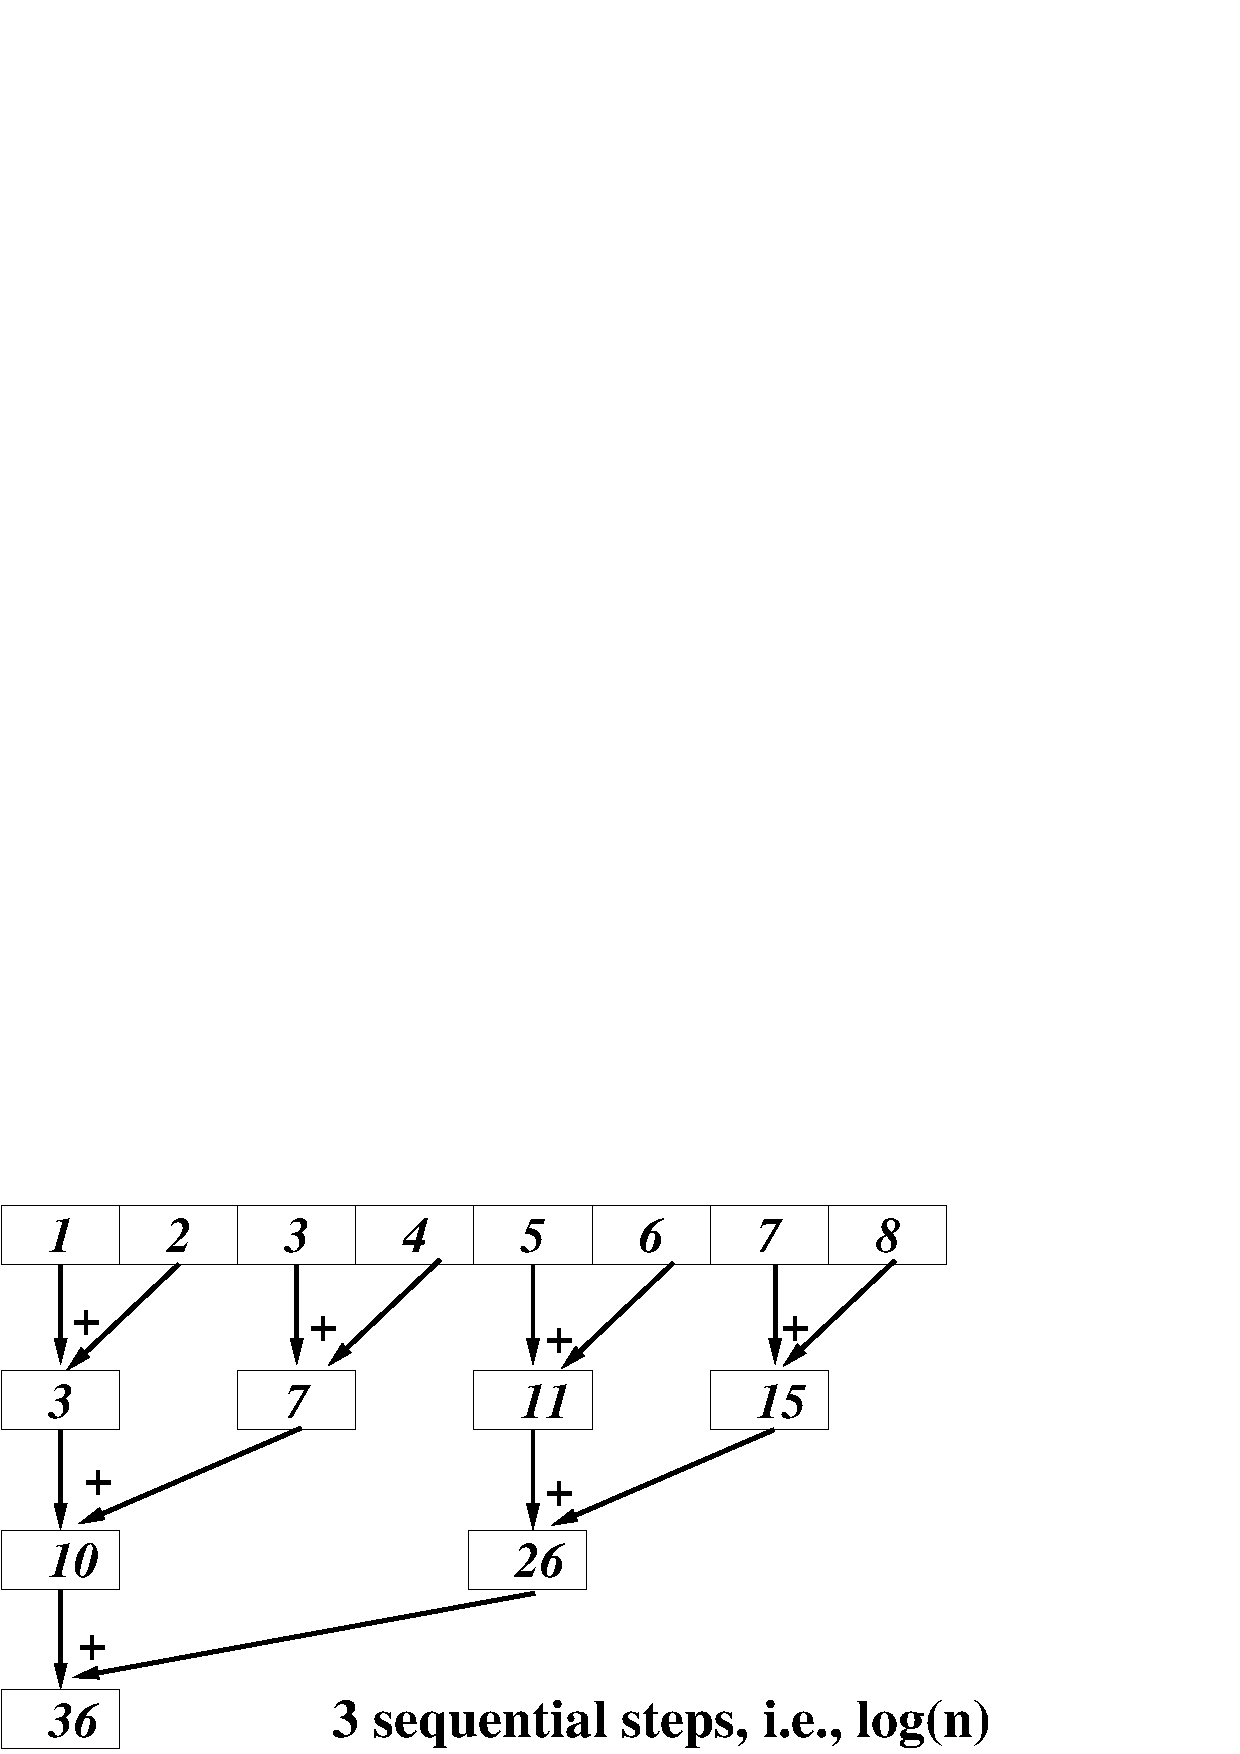
\includegraphics[height=22ex]{Figures/L2/ReduceEg.pdf} 
\column{0.5\textwidth}
Reducing an array of length {\tt n} with {\tt  n/2} processors requires:
\begin{itemize}
    \item work $W(n) = n$ and 
    \item depth $D(n) = lg \ n$, i.e., number of sequential steps.
    \item optimized runtime with $P$ processors: \emph{$O(\frac{n}{P} + lg \ P)$.}
\end  {itemize}
\end{columns}

\begin{mytheo}[Brent Theorem]\label{BrentTh}
A Work-Time Algorithm of depth $D(n)$ and work $W(n)$ can be
simulated on a $P$-processor PRAM in time complexity T such that:\\\bigskip
\emp{$\ \ \ \ \ \ \ \ \ \ \ \ \ \ \ \ \frac{W(n)}{P} \leq T < \frac{W(n)}{P} + D(n)$}
\end{mytheo}

\end{frame}


\begin{frame}[fragile,t]
  \frametitle{Reduce: Algorithm and Complexity}


\begin{columns}
\column{0.5\textwidth}
\begin{colorcode}[fontsize=\scriptsize]
Input:  array A of n=2\mymath{\myindu{k}} elems of type T
        \mymath{\oplus : T\times T\rightarrow T} associative
Output: S = \mymath{\oplus\myindx{j=1}\myindu{n} a\myindx{j}}

1.  \emph{forall i = 0 to n-1 do}
2.    B[i] \mymath{\leftarrow} A[i]
3.  \emph{enddo}

4.  \emp{for h = 1 to k do}
5.    \emph{forall i = 0 to n-1 by 2\mymath{\myindu{h}} do} 
6.      B[i] \mymath{\leftarrow} B[i] \mymath{\oplus} B[i+2\mymath{\myindu{h-1}}]
7.    \emph{enddo}
8.  \emp{enddo}
9.  S \mymath{\leftarrow} B[0]  
\end{colorcode}
\column{0.59\textwidth}
\begin{itemize}
    \item $D_{1-3}(n) = \Theta(1)$, $W_{1-3}(n) = \Theta(n)$,
    \item $D_{5-7}(n) = \Theta(1)$, $W_{5-7}(n,h) = \Theta(n/2^h)$,
    \item $D_{4-8}(n) = k \times D_{5-7}(n) = \Theta(lg \ n)$
    \item $W_{4-8}(n) = \sum_{h=1}^k W_{5-7}(n,h) = $\\
          $\Theta(\sum_{h=1}^k (n/2^h) ) = \Theta(n)$
    \item $D_{9}(n) = \Theta(1)$, $W_{9}(n) = \Theta(1)$,\bigskip
    \item \emp{$D(n) = \Theta(lg \ n), W(n) = \Theta(n)$!}
\end{itemize}
\end{columns}
\bigskip

%\mymath{\frac{n}{2\myindu{h}}} do}

\begin{center}  
\emp{$O(\frac{n}{P}) \leq  O(Runtime) < O(\frac{n}{P} + lg \ n)$}
\end{center}


\end{frame}

\begin{frame}[fragile,t]
  \frametitle{Reduce: Naive Implementation in Futhark}

\begin{lstlisting}[mathescape=true]
-- Reduction by hand in Futhark: red-by-hand.fut
-- ==
-- compiled input { [1.0f32, -2.0, 3.0] }
-- output { 2.0f32 }
-- compiled input @ data/f32-arr-16777216.in
-- output { 3091.746094f32 }

let main [n] (a : [n]f32) : f32 = -- assumes n = 2$^k$
  let k = t32 <| f32.log2 <| r32 n
  let b = 
    loop b = a for h < k do
        let n' = n >> (h+1)
        in  map (\i -> unsafe (b[2*i]+b[2*i+1]) ) (iota n')
  in b[0]
\end{lstlisting}

\alert{Performance w.r.t. the native {\tt reduce}?} Compile and Run with:\\
{\tt\$ futhark-opencl red-by-hand.fut}\\
{\tt\$ futhark-dataset --f32-bounds=-1.0:1.0 -g [8388608]f32 | ./red-by-hand -t /dev/stderr}
\end{frame}


\subsection{Implementation of Scan}

\begin{frame}[fragile]
	\tableofcontents[currentsubsection]
\end{frame}

\begin{frame}[fragile,t]
  \frametitle{Map, Reduce, and Scan Types and Semantics}

\begin{itemize}
    \item {\tt \emp{[n]$\alpha$}} denotes the type of an array of \emp{\tt n} elements of type \emp{$\alpha$}.\smallskip
    \item \emp{\tt map~:~($\alpha\rightarrow\beta$)~$\rightarrow$~[n]$\alpha~\rightarrow$~[n]$\beta$}\\
    \emph{\tt map f [x$_1,\ldots, $x$_n$] = [f x$_1$,$\ldots$, f x$_n$]},\\  
        i.e., \emp{\tt{}x$_i$~:~$\alpha, \forall i$}, and 
        \emp{\tt f~:~$\alpha\rightarrow\beta$}.\medskip

    \item \emp{{\tt reduce~:~($\alpha$~$\rightarrow$~$\alpha$~$\rightarrow$~$\alpha$)~$\rightarrow$~$\alpha$~$\rightarrow$~[n]$\alpha$~$\rightarrow$~$\alpha$}}\\
        \emph{\tt reduce $\odot$~e~[x$_1$,x$_2$,..,x$_n$]~=~e$\odot$x$_1\odot$x$_2\odot\ldots\odot$x$_n$},\\
        i.e., \emp{{\tt{}e:$\alpha$, ~~ x$_i$~:~$\alpha, \forall i$}}, and 
        \emp{\tt $\odot$~:~$\alpha\rightarrow\alpha\rightarrow\alpha$}.\medskip

    \item \emp{{\tt scan$^{exc}$~:~($\alpha$~$\rightarrow$~$\alpha$~$\rightarrow$~$\alpha$)~$\rightarrow$~$\alpha$~$\rightarrow$~[n]$\alpha$~$\rightarrow$~[n]$\alpha$}}\\
        \emph{\tt scan$^{exc}~\odot$~e~[x$_1$,$\ldots$,x$_n$]~=~[e,e$\odot$x$_1$,$\ldots$,e$\odot$x$_1\odot\ldots$x$_{n-1}$]}\\
        i.e., \emp{{\tt{}e:$\alpha$, x$_i$~:~$\alpha, \forall i$}}, and 
        \emp{\tt $\odot$~:~$\alpha\rightarrow\alpha\rightarrow\alpha$}.\medskip

    \item \emp{{\tt scan$^{inc}$~:~($\alpha$~$\rightarrow$~$\alpha$~$\rightarrow$~$\alpha$)~$\rightarrow$~$\alpha$~$\rightarrow$~[n]$\alpha$~$\rightarrow$~[n]$\alpha$}}\\
        \emph{\tt scan$^{inc}~\odot$~e~[x$_1$,$\ldots$,x$_n$]~=~[e$\odot$x$_1$,$\ldots$,e$\odot$x$_1\odot\ldots$x$_{n}$]}\\
        i.e., \emp{{\tt{}e:$\alpha$, x$_i$~:~$\alpha, \forall i$}}, and 
        \emp{\tt $\odot$~:~$\alpha\rightarrow\alpha\rightarrow\alpha$}.

\end{itemize}

\end{frame}



\begin{frame}[fragile,t]
  \frametitle{Parallel Exclusive Scan with Associative Operator $\oplus$}
\bigskip

\begin{columns}
\column{0.4\textwidth}
        \includegraphics[height=33ex]{Figures/L2/ScanEg.pdf} 
\column{0.6\textwidth}
Two Steps:
\begin{itemize}
    \item \blue{Up-Sweep:} similar with reduction
    \item Root is replaced with neutral element.
    \item \emp{Down-Sweep:} 
    \begin{itemize}
        \item the left child sends its value to parent and 
                updates its value to that of parent.
        \item the right-child value is given by $\oplus$ 
                applied to the left-child value and
                the (old) value of parent.
        \item note that the right child is in fact the parent,
                i.e., in-place algorithm.
    \end  {itemize}
\end  {itemize}
\end{columns}


\end{frame}



\begin{frame}[fragile,t]
  \frametitle{Parallel Exclusive Scan Algorithm And Complexity}
\bigskip

\begin{columns}
\column{0.5\textwidth}
\begin{colorcode}[fontsize=\scriptsize]
Input:  array A of n=2\mymath{\myindu{k}} elems of type T
        \mymath{\oplus::T\times T\rightarrow T} associative
Output: B = \mymath{[0, a\myindx{1}, a\myindx{1}\oplus{}a\myindx{2},\ldots,\oplus\myindx{j=1}\myindu{n-1} a\myindx{j}]}

1.  \emph{forall i = 0 : n-1 do}
2.    B[i] \mymath{\leftarrow} A[i]
3.  \emph{enddo}

4.  \emp{for d = 0 to k-1 do} \emph{// up-sweep}
5.    \emph{forall i = 0 to n-1 by 2\mymath{\myindu{d+1}} do} 
6.      B[i+2\mymath{\myindu{d+1}}-1] \mymath{\leftarrow} B[i+2\mymath{\myindu{d}}  -1] \mymath{\oplus} 
                       B[i+2\mymath{\myindu{d+1}}-1]
7.    \emph{enddo}
8.  \emp{enddo}
9.  B[n-1] = 0
10. \emp{for d = k-1 downto 0 do} \emph{// down-sweep}
11.   \emph{forall i = 0 to n-1 by 2\mymath{\myindu{d+1}} do} 
12.     tmp \mymath{\leftarrow} B[i+2\mymath{\myindu{d}}-1]
13.     B[i+2\mymath{\myindu{d}}-1] \mymath{\leftarrow} B[i+2\mymath{\myindu{d+1}}-1]
14.     B[i+2\mymath{\myindu{d+1}}-1] \mymath{\leftarrow} tmp \mymath{\oplus} B[i+2\mymath{\myindu{d+1}}-1]
15.   \emph{enddo}
16. \emp{enddo}
\end{colorcode}
\column{0.59\textwidth}
\begin{itemize} 
    \item The code show exponentials for clarity, but those can
            be computed by one multiplication/division operation
            each sequential iteration.
    \item \emp{$D(n) = \Theta(lg \ n), W(n) = \Theta(n)$!}
    \item Similar reasoning as with reduce.
\end{itemize}
\end{columns}

%4.  \emp{for h = 1 to k do} // up-sweep
%5.    \emph{forall i \mymath{\in} n : 1 by -2\mymath{\myindu{h}} do} 
%6.      B[i] \mymath{\leftarrow} B[i] \mymath{\oplus} B[i-2\mymath{\myindu{h-1}}]
%7.    \emph{enddo}
%8.  \emp{enddo}
%9.  B[n] = 0
%
%10. \emp{for h = k downto 1 do} // down-sweep
%11.   \emph{forall i \mymath{\in} n : 1 by -2\mymath{\myindu{h}} do} 
%12.     tmp = B[i]
%13.     B[i] \mymath{\leftarrow} B[i] \mymath{\oplus} B[i-2\mymath{\myindu{h-1}}]
%14.     B[i-2\mymath{\myindu{h-1}}] = tmp
%15.   \emph{enddo}
%16. \emp{enddo}


\end{frame}

%%%%%%%%%%%%%%%%%%%%%%%%%%%%%%%%%%%%%%%%%
%%%%%%%%%%%%%%%%%%%%%%%%%%%%%%%%%%%%%%%%%

\subsection{Implementation of Segmented Scan}

\begin{frame}[fragile]
	\tableofcontents[currentsubsection]
\end{frame}

\begin{frame}[fragile,t]
  \frametitle{{\scriptsize Slide from CMU 15-418: Parallel Computer Architecture and Programming (Spring 2012)}}
\vspace{-3ex}
\begin{center}
\includegraphics[height=50ex]{Figures/L2/SegmExclScan} 
\end  {center}

\end{frame}


\begin{frame}[fragile,t]
  \frametitle{Segmented Exclusive Scan Alg And Complexity}
\vspace{-2ex}
\begin{columns}
\column{0.6\textwidth}
\begin{colorcode}[fontsize=\scriptsize]
Input:  flag array F of n=2\mymath{\myindu{k}} of ints
        data array A of n=2\mymath{\myindu{k}} elems of type T
        \mymath{\oplus::T\times T\rightarrow T} associative
Output: B = segmented scan of 2-dim array A
1.  \emph{FORALL i = 0 to n-1 do} B[i] \mymath{\leftarrow} A[i] \emph{ENDDO}
2.  \emp{FOR d = 0 to k-1 DO} \emph{// up-sweep}
3.    \emph{FORALL i = 0 to n-1 by 2\mymath{\myindu{d+1}} DO} 
4.      IF F[i+2\mymath{\myindu{d+1}}-1] == 0 THEN 
5.          B[i+2\mymath{\myindu{d+1}}-1] \mymath{\leftarrow} B[i+2\mymath{\myindu{d}}-1] \mymath{\oplus} B[i+2\mymath{\myindu{d+1}}-1]
6.      ENDIF
7.      F[i+2\mymath{\myindu{d+1}}-1] \mymath{\leftarrow} F[i+2\mymath{\myindu{d}}-1] .|. F[i+2\mymath{\myindu{d+1}}-1]
8.  \emp{ENDDO} \emph{ENDDO}
9.  B[n-1] \mymath{\leftarrow} 0
10. \emp{FOR d = k-1 downto 0 DO} \emph{// down-sweep}
11.   \emph{FORALL i = 0 to n-1 by 2\mymath{\myindu{d+1}} DO} 
12.     tmp \mymath{\leftarrow} B[i+2\mymath{\myindu{d}}-1]
13.     IF \alert{F\_original}[i+2\mymath{\myindu{d}}] \mymath{\neq} 0 THEN
14.          B[i+2\mymath{\myindu{d+1}}-1] \mymath{\leftarrow} 0
15.     ELSE IF F[i+2\mymath{\myindu{d}}-1] \mymath{\neq} 0 THEN
16.          B[i+2\mymath{\myindu{d+1}}-1] \mymath{\leftarrow} tmp
17.     ELSE B[i+2\mymath{\myindu{d+1}}-1] \mymath{\leftarrow} tmp \mymath{\oplus} B[i+2\mymath{\myindu{d+1}}-1]
18.     ENDIF
19.     F[i+2\mymath{\myindu{d+1}}-1] \mymath{\leftarrow} 0
20. \emp{ENDDO} \emph{ENDDO}
\end{colorcode}
\column{0.35\textwidth}
\begin{itemize} 
    \item While there are more branches, the asymptotics 
            does not change:
    \item \emph{$D(n) = \Theta(lg \ n)$},\\\emp{$W(n) = \Theta(n)$!}
\end{itemize}
\end{columns}

\end{frame}


\begin{frame}[fragile,t]
  \frametitle{Segmented Inclusive Scan with Operator $\oplus$ (Haskell)}

\emphh{Equiv with Mapping a Scan op on each segment of an irregular array.}

\begin{columns}
\column{0.55\textwidth}
\begin{colorcode}
-- iota n = [0..n-1]
map (\mymath{\backslash}i-> scan (+) 0 [1..i]) [3,4] \emph{\mymath{\equiv}}\pause
[ scan\mymath{\myindu{inc}} (+) 0 [1,2,3], 
  scan\mymath{\myindu{inc}} (+) 0 [1,2,3,4] ] 
      \emph{\mymath{\equiv}}
[ [1,3,6], [1,3,6,10] ]
\end{colorcode}
\column{0.55\textwidth}
\begin{colorcode}
-- \blue{Flags \& Flat Data Representation:}
sgmScanInc (+) 0 [1,0,0,1,0,0,0] -- \emph{flag}
                 [1,2,3,1,2,3,4] -- \emp{data}
    \emph{\mymath{\equiv}}

  [1,3,6,1,3,6,10]        -- \emp{scanned data}
\end{colorcode}
\end{columns}
\medskip

%( [1,0,0,1,0,0, 0],              -- \emph{flag}


\emphh{Can be obtained by replacing the following Futhark operator:}
\smallskip

\begin{lstlisting}[mathescape=true]
let segmented_scan [n] 't (op: t -> t -> t) (ne: t)
                       (flags: [n]bool) (arr: [n]t) : [n]t =
  let (_, res) = unzip <|
    scan (\(x_flag,x) (y_flag,y) ->
             let fl = x_flag || y_flag
             let vl = if y_flag then y else x `op` y
             in  (fl, vl)
         ) (false, ne) (zip flags arr)
  in  res
\end{lstlisting}\vspace{-2ex}

\bigskip

\alert{How about Exclusive Scan?}

\end{frame}

%%%%%%%%%%%%%%%%%%%%%%%%%%%%%%%%%%%%%%%%%
%%%%%%%%%%%%%%%%%%%%%%%%%%%%%%%%%%%%%%%%%
\subsection{Other Second-Order Parallel Operators}

\begin{frame}[fragile]
	\tableofcontents[currentsubsection]
\end{frame}


\begin{frame}[fragile,t]
  \frametitle{Zip, Unzip, Map2, Filter}

\begin{itemize}
    \item \emph{\tt zip : [n]$\alpha_1$ $\rightarrow$ [n]$\alpha_2$ $\rightarrow$ [n]($\alpha_1$,$\alpha_2$)}
    \item \emp{\tt zip [a$_1$,$\ldots$,a$_n$] [b$_1$,$\ldots$,b$_n$] $\equiv$ [(a$_1$,b$_1$),\ldots,(a$_n$,b$_n$)]},\pause
    \item \emph{\tt unzip : [n]($\alpha_1$,$\alpha_2$) $\rightarrow$ ([n]$\alpha_1$,[n]$\alpha_2$)}
    \item \emp{\tt unzip [(a$_1$,b$_1$),\ldots,(a$_n$,b$_n$)]$\equiv$([a$_1$,$\ldots$,a$_n$],[b$_1$,$\ldots$,b$_n$])},
    \item In some sense {\tt zip/unzip} are syntactic sugar

    \item {\tt map2 : ($\alpha_1\rightarrow\alpha_2\rightarrow\beta$) $\rightarrow$ [n]$\alpha_1$ $\rightarrow$ [n]$\alpha_2$ $\rightarrow$ [n]$\beta$}
    \item {\tt map2 $\odot$ [a$_1$,$\ldots$,a$_n$] [b$_1$,$\ldots$,b$_n$] $\equiv$ [a$_1\odot$b$_1$,$\ldots$,a$_n\odot$b$_n$]}
    \item {\tt map3 $\ldots$}\medskip\pause

    \item {\tt filter : ($\alpha$ $\to$ Bool) $\to$ [n]$\alpha$ $\to$ [m]$\alpha$}   (where {\tt m $\leq$ n})
    \item {\tt filter p [a$_1$, $\ldots$, a$_n$] = [a$_{k_1}$,$\ldots$, a$_{k_m}$]} such that\\
        {\tt k$_1$ < k$_2$ < $\ldots$ < k$_m$}, and denoting by $\overline{\mbox{\tt k}}$ = {k$_1$,$\ldots$, k$_m$}, we have\\
        {\tt(p a$_j$ == true)} $\forall$ $j~\in~\overline{\mbox{\tt k}}$, \textbf{and} {\tt(p a$_j$ == false)} $\forall$ $j~\not\in~\overline{\mbox{\tt k}}$.\medskip
\end  {itemize}

Note: in Haskell {\tt zip,map2} do not expect same-length arrays;\\ in Futhark they do!

\end{frame}

\begin{frame}[fragile,t]
  \frametitle{Scatter: A Parallel Write Operator}

Scatter \emph{updates in parallel} a base array with a set of values at specified indices:
\smallskip

\emph{scatter : *[m]$\alpha$ $\rightarrow$ [n]int $\rightarrow$ [n]$\alpha$ $\rightarrow$ *[m]$\alpha$}
\bigskip

A (data vector)    {\tt~=[b0, b1, b2, b3]}\\
I (index vector)   {\tt~=[2,~~4,~~1,~~-1]}\\
X (input array)    {\tt~=[a0,~a1,~a2,~a3,~a4,~a5]}\\
\emp{scatter X I A {\tt~~~=[a0,~b2,~b0,~a3,~b1,~a5]}}
\bigskip\pause

\emph{scatter} has $D(n)=\Theta(1)$ and $W(n)=\Theta(n)$,\\
i.e., requires {\tt n} update operations ({\tt n} is the size of I or A, not of X!). 
\smallskip 

\begin{itemize}
\item[1] \emp{Array X is consumed by {\tt scatter}; following uses of X are illegal!}\\
\item[2] \emp{Similarly, X can alias neither I nor A!}
\end{itemize}
\smallskip 

In Futhark, {\tt scatter} check and ignores the indices that are out of bounds (no update is performed on those).
This is useful for padding the iteration space in order to obtain regular parallelism. 
\end{frame}

\begin{frame}[fragile,t]
  \frametitle{Permute, Split, Replicate, Iota}

\begin{itemize}
    \item Operator to \emph{permute in parallel} based on a set (array) of indices:\\
          \emph{permute : [n]int$\rightarrow$[n]$\alpha$$\rightarrow$[n]$\alpha$}. 
          {\small~\blue{\tt permute~I~A~$\equiv$~scatter~(replicate n e)~I~A}}\\
           A (data vector) {\tt~= [a0,~a1,~a2,~a3,~a4,~a5]}\\
           I (index vector){\tt~~= [3,~~2,~~0,~~4,~~1,~~5~]}\\
           \emp{permute I A     {\tt~~~~= [a2,~a4,~a1,~a0,~a3,~a5]}}\\\bigskip
           
    \item %Operator to {\tt split} a list (array) at a certain index:\\
          \emph{\tt split : (i:int) $\rightarrow$ [n]$\alpha$ $\rightarrow$ ([i]$\alpha$,[n-i]$\alpha$)}\\
          \emp{\tt split i [a$_0$,$\ldots$,a$_{n-1}$] $\equiv$ ([a$_0$,$\ldots$,a$_{i-1}$], [a$_i$,$\ldots$,a$_{n-1}$])}\smallskip

    \item \emph{\tt replicate : (n:int) $\rightarrow$ $\alpha$ $\rightarrow$ [n]$\alpha$}\\
            \emp{\tt replicate n a $\equiv$ [a, a,$\ldots$, a]}, i.e., {\tt a} is replicated {\tt n} times.\smallskip

    \item \emph{\tt iota : (n:int) $\rightarrow$ [n]int}\\
             \emp{\tt iota n = [0,$\ldots$,n-1]}
\end  {itemize}

\end{frame}

\begin{frame}[fragile,t]
  \frametitle{Partition2/Filter Implementation}

%\mymath{\backslash}

\emph{\tt partition2 : ($\alpha\rightarrow$Bool) $\rightarrow$ [n]$\alpha$ $\rightarrow$ ([n]i32,[n]$\alpha$)}\\
In result, the elements satisfying the predicate occur before the others.
%\emp{\tt filter cond X $\equiv$ [b$_0$,$\ldots$,b$_{m}$]}, such that 
%{\tt b$_j, \forall j\in\{0\ldots m\}$,} are all the elements of array 
%{\tt X} that evaluate to {\tt True} under condition {\tt cond}, i.e., {\tt (cond b$_j$) $\equiv$ True}.\medskip

\emp{Can be implemented by means of {\tt map}, {\tt scan} and {\tt scatter}.}\pause


\begin{columns}
\column{0.59\textwidth}
  \lstset{basicstyle=\scriptsize}
  \begin{lstlisting}
let partition2 [n] (X : [n]i32) : 
              ([n]i32, [n]i32) =
 let cs = map cond X
 let tfs= map (\ f->if f then 1 
                         else 0) cs
 let isT= scan (+) 0 tfs
 let i  = isT[n-1]

 let ffs= map (\f->if f then 0 
                        else 1) cs
 let isF= map (+i) (scan (+) 0 ffs)
 let inds=map (\(c,iT,iF) -> 
                  if c then iT-1 
                       else iF-1
              ) (zip cs isT isF)
 let flags = scatter (replicate n 0) 
                     [0,i] [i,n-i]
 in (scatter (replicate n 0) inds X, flags)
\end{lstlisting}
  \lstset{basicstyle=\small}
\column{0.4\textwidth}\vspace{-2ex}
\begin{colorcode}[fontsize=\scriptsize]
Assume X = [5,4,2,3,7,8], and 
cond is T(rue) for even nums.\pause
n   = 6
cs  = [F, T, T, F, F, T]
tfs = [0, 1, 1, 0, 0, 1]

isT = [0, 1, 2, 2, 2, 3]
i   = 3

ffs = [1, 0, 0, 1, 1, 0]
isF = [4, 4, 4, 5, 6, 6]

inds= [3, 0, 1, 4, 5, 2]


flags  = [3, 0, 0, 3, 0, 0]
Result = [4, 2, 8, 5, 3, 7] 
\end{colorcode}
\end{columns}

\end{frame}


%%%%%%%%%%%%%%%%%%%%%%%%%%%%%%%%%%%%%%%%%%%%%
%%%%%%%%%%%%%%%%%%%%%%%%%%%%%%%%%%%%%%%%%%%%%
%%%%%%%%%%%%%%%%%%%%%%%%%%%%%%%%%%%%%%%%%%%%%


\section{Nested Data-Parallel Applications} 

\begin{frame}[fragile]
	\tableofcontents[currentsection]
\end{frame}

\subsection{Sieve: Prime-Numbers Computation}

\begin{frame}[fragile,t]
  \frametitle{Computing Prime Numbers: First Attempt}

See also "Scan as Primitive Parallel Operation" [Bleelloch]\\
(attached in Additional Teaching Material module).

\medskip

Start with an array of size $n$ filled initially with $1$,
i.e., all are primes, and iteratively zero out all multiples
of numbers up to $\sqrt{n}$.
\bigskip

\begin{colorcode}
int res[n] = \{0, 0, 1, 1, 1, ..., 1\}
for(i = 2; i < sqrt(n); i++) \{  \alert{//sequential}
    if ( res[i] != 0 ) \{
        \emph{forall m \mymath{\in multiples of i \leq n} do} \{
             res[m] = 0;
        \}
    \}
\}
\end{colorcode}
\bigskip

\emph{Work: $O(n \ lg \ lg \ n)$} but \emp{Depth: $O(\sqrt{n})$ (Not Good Enough!)}

\end{frame}

\begin{frame}[fragile,t]
  \frametitle{Computing Prime Numbers: 1st Attempt (Futhark)}

Start with an array of size $n$ filled intially with $1$,
i.e., all are primes, and iteratively zero out all multiples
of numbers up to $\sqrt{n}$.

\begin{columns}
\column{0.59\textwidth}

\lstset{basicstyle=\scriptsize}
  \begin{lstlisting}
let primesHelp [np1] (sq : i32) 
        (a : *[np1]i32) : [np1]i32 =
 let n = np1 - 1 in
 loop(a) for j < (sq-1) do 
   let i   = j + 2
   let m   = (n / i) - 1
   let inds= map (\k->(k+2)*i)(iota m)
   in  scatter a inds (replicate m 0)

let main (n : i32) : []i32 = 
  let a = map (\i->if i==0 || i==1
                   then 0 else 1) 
              (iota (n+1))
  let sq= i32 (f32.sqrt (f32 n))
  let fl= primesHelp sq a
  in  filter (\i->unsafe fl[i]!=0) 
             (iota (n+1))
  \end{lstlisting}
\lstset{basicstyle=\small}
%
\column{0.4\textwidth}
\vspace{-2ex}
\begin{colorcode}[fontsize=\scriptsize]
Assume n = 9, sqrtN = 3 
a = [0,0,1,1,1,1,1,1,1,1]

iteration j = 0, i = 2
m    = (9 `div` 2) - 1 = 3
inds = [4, 6, 8]
vals = [0, 0, 0]
a' = [0,0,1,1,\emp{0},1,\emp{0},1,\emp{0},1]

iteration j = 1, i = 3
m    = (9 `div` 3) - 1 = 2
inds = [6, 9]
vals = [0, 0]
a''= [0,0,1,1,0,1,\emp{0},1,0,\emp{0}]

iteration j = 2, i = 4
result: [0,0,\emp{1},\emp{1},0,\emp{1},0,\emp{1},0,\emp{0}]
  i.e., [0,1,\emp{2},\emp{3},4,\emp{5},6,\emp{7},8,9]
\end{colorcode}
\end{columns}
\medskip

\emph{Work: $O(n \ lg \ lg \ n)$} but \emp{Depth: $O(\sqrt{n})$ (Not Good Enough!)}

\end{frame}


\begin{frame}[fragile,t]
  \frametitle{Prime Numbers: Nested Parallelism in Haskell}
\vspace{-2ex}
If we have all primes from $2$ to $\sqrt{n}$ we could
generate all multiples of these primes at once:
\emp{\tt \{[2*p:n:p]: p in sqr\_primes\}} in NESL.
\blue{Also call algorithm recursively on $\sqrt{n}$ $\Rightarrow$ Depth: $O(lg \ lg \ n)$!}\\
(solution of $n^{(1/2)^{depth}}=2$).
\pause
\begin{columns}
\column{0.59\textwidth}
\begin{colorcode}[fontsize=\scriptsize]
primesOpt :: Int -> [Int]
primesOpt n = 
  if n <= 2 then [2]
  else 
   let sqrtN = floor (sqrt (fromIntegral n))
       \blue{sqrt_primes = primesOpt sqrtN}
       nested = \emp{map} (\mymath{\backslash}\emp{p}->let m = (n `div` p) 
                         in  \emp{map} (\mymath{\backslash}j-> j*p)
                                 [2..m]
                    ) \emp{sqrt_primes}
       not_primes  = \emph{reduce} (++) [] nested
       mm = length not_primes
       zeros = \emph{replicate} mm False 
       prime_flags=\emph{scatter}\emph{(replicate} (n+1) True) 
                            not_primes zeros 
       (primes,_)= unzip $ \emph{filter} (\mymath{\backslash}(i,f)->f) 
                    $ (zip [0..n] prime_flags)
   in drop 2 primes
\end{colorcode}
\column{0.4\textwidth}\pause
\begin{colorcode}[fontsize=\scriptsize]
Assume n = 9, sqrtN = 3 

call primesOpt 3
n = 3,sqrtN = 1,sqrt_primes=[2]
nested = [[]]; not\_primes = [] 
mm = 0; zeros = []
prime_flags = [T,T,T,T]
primes = [0,1,2,3]; returns [2,3]

in primesOpt 9, afer 
return from primesOpt3,
sqrt_primes = [2,3]
nested = [[4,6,8],[6,9]]
not_primes = [4,6,8,6,9]
mm=5;zeros= [F,F,F,F,F]
prime_flags= [T,T,T,T,\emp{F},T,\emp{F},T,\emp{F},\emp{F}]
primes = [0,1,2,3,5,7]
returns [2,3,5,7]
\end{colorcode}
\end{columns}

\end{frame}

\subsection{Nested Parallel Quicksort}

\begin{frame}[fragile,t]
  \frametitle{Quicksort with Nested Parallelism}

\begin{columns}
\column{0.59\textwidth}
\begin{colorcode}[fontsize=\scriptsize]
nestedQuicksort :: [a] -> [a]
nestedQuicksort arr = 
  if (length arr) <= 1 then arr else 
  let i = getRand (0, (length arr) - 1)
      a = arr !! i
      s1 = filter (\mymath{\backslash}x -> (x <  a)) arr
      s2 = filter (\mymath{\backslash}x -> (x >= a)) arr
      rs = map nestedQuicksort [s1, s2]
  in  (rs !! 0) ++ (rs !! 1)

-- \alert{Is this implementation correct?}
-- \alert{Average Depth and Work ?}
\end{colorcode}
\column{0.4\textwidth}\pause
\begin{colorcode}[fontsize=\scriptsize]
Assume input array [3,2,4,1]
Assume random i = 0 \mymath{\Rightarrow} a = 3

s1 = [2,1]
s2 = [3,4]

\emp{nestedQuicksort [2,1]}:
i = 0, a = 2
s1 = [1]
s2 = [2]
results in [1]++[2]==[1,2]

\emp{nestedQuicksort [3,4]}: ...
results in [3,4]

\emp{After recursion concat:}
[1,2] ++ [3,4] = [1,2,3,4]
\end{colorcode}
\end{columns}
\medskip

Denoting by $n$ the size of the input array: Average Work is $O(n \ lg \ N)$.\\
\medskip

If filter would have depth $1$, then Average Depth: $O(lg \ n)$.
\medskip

In practice we have depth: $O(lg^2 \ n)$.

\end{frame}

\section{Flattening Nested Parallelism}

\begin{frame}[fragile]
	\tableofcontents[currentsection]
\end{frame}

\subsection{Rules For Flattening}

\begin{frame}[fragile,t]
  \frametitle{Nested {\it vs} Flattened Parallelism: Scan inside a Map}

\blue{\bf (1) Scan inside a nested map:}

\begin{colorcode}[fontsize=\scriptsize]
map (\mymath{\backslash}row->scan\mymath{\myindu{inc}} (+) 0 row) \emp{[[1,3], [2,4,6]]} 
\mymath{\equiv}
[ scan\mymath{\myindu{inc}} (+) 0 [1,3],    scan\mymath{\myindu{inc}} (+) 0 [2,4,6] ] 
\mymath{\equiv}
\emp{[ [ 1, 4],               [2, 6, 12] ]}
\end{colorcode}

\bigskip
\pause

\blue{\bf becomes a segmented scan}, which requires a flag array as arg:
\bigskip

\begin{colorcode}[fontsize=\scriptsize]
sgmScan\mymath{\myindu{inc}} (+) 0 \emph{[2, 0, 3, 0, 0]} \emph{[1, 3, 2, 4, 6]} \mymath{\equiv} \emph{[ 1, 4, 2, 6, 12 ]}
\end{colorcode}

\bigskip

The flag array \emph{[2, 0, 3, 0, 0]} encodes the fact that the 
flat-data array \emph{[1, 3, 2, 4, 6]} has two segments:
\begin{itemize} 
    \item one of length $2$ starting at index $0$
    \item one of length $3$ starting at index $2$
\end{itemize}

(i.e., an non-zero element in the flag array denotes the 
       length of the segment that start at that point.  )

\end{frame}

\begin{frame}[fragile,t]
  \frametitle{Nested {\it vs} Flattened Parallelism: Map inside a Map}

\blue{\bf (2) Map nested inside a map:}

\begin{colorcode}[fontsize=\scriptsize]
map (\mymath{\backslash}row->map f row) \emp{[[1,3], [2,4,6]]} 
\mymath{\equiv}
[ map f [1, 3],      map f [2, 4, 6] ] 
\mymath{\equiv}
\emp{[ [f(1),f(3)], [f(2),f(4),f(6)] ]}
\end{colorcode}

\bigskip
\pause

\blue{\bf becomes a map on the flat array:}
\bigskip

\begin{colorcode}[fontsize=\scriptsize]
map f \emph{[1, 3, 2, 4, 6]} \mymath{\equiv} \emph{[ f(1), f(3), f(2), f(4), f(6) ]}
\end{colorcode}

\bigskip

The flag array is assumed known and is preserved \emph{[2, 0, 3, 0, 0]}

\end{frame}

\begin{frame}[fragile,t]
  \frametitle{How To Distribute the Segment Size?}

Assume flag array: \emph{\tt [2, 0, 3, 0, 0]}.

\bigskip

How do we get \emp{\tt [2, 2, 3, 3, 3]}?

\bigskip
\pause

\blue{\tt sgmScan\mymath{\myindu{inc}} (+) 0 flags flags}

\end{frame}


\begin{frame}[fragile,t]
  \frametitle{Nested {\it vs} Flattened Parallelism: Replicate in a Map}

\blue{\bf (4) Replicate nested inside a map:}

\begin{colorcode}[fontsize=\scriptsize]
map (\mymath{\backslash}(n,m) -> replicate n m) \emp{[(1,7),(3,8),(2,9)]} \mymath{\equiv}
[ replicate 1 7, replicate 3 8, replicate 2 9 ] \mymath{\equiv}
[ [7], [8,8,8], [9,9] ]
\end{colorcode}

\bigskip
\pause

\blue{\bf becomes a composition of scans and scatter:}
\bigskip

\begin{colorcode}[fontsize=\scriptsize]
1. (ns, ms)  = unzip([(1,7), (3,8), (2,9)]      -- ([1,3,2], [7,8,9])
2. inds = scan\mymath{\myindu{exc}} (+) 0 ns                       -- [0,1,4]
3. size = (last inds) + (last ns)               -- 4 + 2 = 6
5. flag = scatter (replicate size 0) inds  ms   -- [7, 8, 0, 0, 9, 0]
6. sgmScan\mymath{\myindu{inc}} (+) 0 flag \emp{flag}                    \emph{-- [7, 8, 8, 8, 9, 9]}
\end{colorcode}

\bigskip

\begin{itemize}
    \item[2.] builds the indices at which segment start
    \item[3.] get the size of the flat array (equivalent to summing {\tt ns})
    \item[4-5.] write the array elems at the position where a segment starts
    \item[6.] distribute the start-elem of a segment throughout the segment. 
    \item \alert{Implementation shortcomings:} \pause replicate 0 7? \pause sgmScan\mymath{\myindu{inc}} (+)?
\end{itemize}

\end{frame}


\begin{frame}[fragile,t]
  \frametitle{Nested {\it vs} Flattened Parallelism: Iota in a Map}

\blue{\bf (5) Iota nested inside a map} ({\tt (iota n)$\equiv$[0,$\ldots$,n-1]}): 

\begin{colorcode}[fontsize=\scriptsize]
map (\mymath{\backslash}i -> iota i) \emp{[1,3,2]} \mymath{\equiv}
[ iota 1, iota 3, iota 2 ] \mymath{\equiv} [ [0], [0,1,2], [0,1] ]
\end{colorcode}

\medskip
\pause

\blue{\bf becomes a composition of scans and scatter:}\\
Note that {\tt iota n $\equiv$ scan$^{exc}$ (+) 0 (replicate n 1)}

\medskip

\begin{colorcode}[fontsize=\scriptsize]
1. arr  = [1, 3, 2]
2. inds = scan\mymath{\myindu{exc}} (+) 0 arr         -- [0,1,4]
3. size = (last inds) + (last arr) -- 4 + 2 = 6
4. flag = scatter (replicate size 0)
                  inds  -- \emp{[0,1,4]}
                  arr   -- \emp{[1,3,2]}
--                [1, 3, 0, 0, 2, 0]
5. \emp{tmp  = replicate size 1  --[1, 1, 1, 1, 1, 1]}
6. sgmScan\mymath{\myindu{exc}} (+) 0 flag \emp{tmp} \emph{--[0, 0, 1, 2, 0, 1]}
\end{colorcode}

\medskip

\begin{itemize}
    \item[2.] builds the indices at which segment start
    \item[3.] get the size of the flat array (equivalent to summing {\tt arr})
    \item[4.] write the array elems at the position where a segment starts
    \item[6.] \emp{segmented scan an array of ones}.
\end{itemize}

\end{frame}




\begin{frame}[fragile,t]
  \frametitle{Nested {\it vs} Flattened Parallelism: If Inside a Map}

\blue{\bf (6) An If-Then-Elese with inner parallelism nested inside a map:} 

\begin{colorcode}[fontsize=\scriptsize]
let arr = [3, 4, 6, 7] in
map(\mymath{\backslash}x -> if (odd x)  then f x  -- assume f is *2
                      else g x  -- assume g is -1 ) arr 
-- should result in [6, 3, 5, 14]
\end{colorcode}

\bigskip
\pause

\textbf{\blue{translates to a} \emp{scatter-}\emph{map}\purple{-gather} \blue{composition}:}
\bigskip

\begin{colorcode}[fontsize=\scriptsize]
1. ais = zip arr (iota (length arr))      -- [(3,0), (4,1), (6,2), (7,3)]
2. (ais',flg)=\emp{partition2}(\mymath{\backslash}(x,_)->odd x) ais--([(3,0),(7,3),(4,1),(6,2)],[2,0,2,0])
3. (ais\mymath{\myindu{t}},ais\mymath{\myindu{f}}) = split flg[0] ais'        --([(3,0),(7,3)], [(4,1),(6,2)])
4. (arr\mymath{\myindu{t}},inds\mymath{\myindu{t}}) = unzip ais\mymath{\myindu{t}}                 --([3,7], [0,3])
5. (arr\mymath{\myindu{f}},inds\mymath{\myindu{f}}) = unzip ais\mymath{\myindu{f}}                 --([4,6], [1,2])
6. (arr\mymath{\myindu{then}},arr\mymath{\myindu{else}}) = (\emph{map f arr\mymath{\myindu{t}}, map g arr\mymath{\myindu{f}}}) --([6,14], [3,5])
7. result = \purple{scatter (scatter [0,\mymath{\ldots},0] inds\mymath{\myindu{t}} arr\mymath{\myindu{then}}) inds\mymath{\myindu{f}} arr\mymath{\myindu{else}}} --[6, 3, 5, 14]
\end{colorcode}

\bigskip

\begin{itemize}
    \item[1-2.] zip array with indices and \emp{permute based on if predicate},
    \item[3-5.] unzip the array segments and indices,
    \item[6.] \emph{map the two data arrays}
    \item[7.] \purple{write back the resulted elements at original positions.}
\end{itemize}

\end{frame}


\begin{frame}[fragile,t]
  \frametitle{Nested {\it vs} Flattened Parallelism: Reduce Inside Map}

\blue{\bf (7) Reduce Inside a Map or Segmented Reduce:} 

\begin{colorcode}[fontsize=\scriptsize]
let arr = [[1, 3, 4], [6, 7]] in
map (\mymath{\backslash}x -> reduce + 0 x) arr 
-- should result in [8, 13]
\end{colorcode}

\bigskip
\pause

\textbf{\blue{translates to a} \emp{scan-}\emph{pack} \blue{composition}:}
\bigskip

\begin{colorcode}[fontsize=\scriptsize]
1. shp    = [3, 2]
2. flags  = [1, 0, 0, 1, 0]
3. arr    = [1, 3, 4, 6, 7]
4. n      = length arr
5. indsp1 = scan\mymath{\myindu{inc}} (+) 0 shp          -- [3, 5] 
6. sc_arr = \emp{sgmScan\mymath{\myindu{inc}}} (+) 0 flags arr -- [1, 4, 8, 6, 13]
7. res    = map (\mymath{\backslash} ip1 -> sc_arr[ip1-1]) indsp1
\end{colorcode}

\end{frame}


%%%%%%%%%%%%%%%%%%%%%%%%%%%%%%%%%%%%%%%%%%%%%%%%%%%%%%%%%%%%%%%%%%%%%%%%%%%%
%%%%%%%%%%%%%%%%%%%%%%%%%%%%%%%%%%%%%%%%%%%%%%%%%%%%%%%%%%%%%%%%%%%%%%%%%%%%
%%%%%%%%%%%%%%%%%%%%%%%%%%%%%%%%%%%%%%%%%%%%%%%%%%%%%%%%%%%%%%%%%%%%%%%%%%%%

\subsection{Flattening a Simple (Contrived) Program}

\begin{frame}[fragile]
	\tableofcontents[currentsubsection]
\end{frame}


\begin{frame}[fragile,t]
  \frametitle{How to Flatten? A Relatively Simple Case}
\begin{colorcode}
let arr = [1, 2, 3, 4] in
\alert{map (\mymath{\backslash}i -> map (+(i+1)) (iota i)) arr}
-- Result: [[2],[3,4],[4,5,6],[5,6,7,8]]
\end{colorcode}
\bigskip
\pause

Normalize the code:
\begin{colorcode}
map (\mymath{\backslash}i -> let ip1 = i+1 in
           let iot = (iota i) in
           let ip1r= (replicate i ip1) in
           map (+) ip1r iot            ) arr
\end{colorcode}
\bigskip

\blue{Distribute the map over every instruction in the body}\\
(bottom-up if nest $>$ 2), where $\mathcal{F}$ denotes the flattening transf,\\
and modify the inputs (results) accordingly.
\bigskip
\pause

\begin{colorcode}
\mymath{\mathcal{F}}(\alert{map (\mymath{\backslash}i -> map (+(i+1)) (iota i)) [0..n-1]}) \mymath{\equiv}
1. let ip1s = map (\mymath{\backslash}i -> i+1) arr in -- [2, 3, 4, 5]
2. let iots = \mymath{\mathcal{F}}(map (\mymath{\backslash}i -> (iota i)) arr)) in
3. let ip1rs= \mymath{\mathcal{F}}(map (\mymath{\backslash}(i,ip1) -> (replicate i ip1)) (zip arr ip1s)))
4. in  \mymath{\mathcal{F}}(map (\mymath{\backslash}(z) -> map (+) z) ip1rs iots)
\end{colorcode}

\end{frame}



\begin{frame}[fragile,t]
  \frametitle{How to Flatten? A Relatively Simple Case}

\blue{\bf According to rule (4) iota nested inside a map}\\
(assuming {\tt arr = [1,2,3,4]}):
\bigskip

\begin{colorcode}
2. let iots = \mymath{\mathcal{F}}(map (\mymath{\backslash}i -> iota(i)) arr)

\mymath{\equiv}

inds = scan\mymath{\myindu{exc}} (+) 0 arr -- [0,1,3,6]
size = (last inds) + (last arr) -- 6 + 4 = 10
flag = scatter (replicate size 0) 
               inds arr
--             [1, 2, 0, 3, 0, 0, 4, 0, 0, 0]
tmp  = replicate size 1
iots = sgmScan\mymath{\myindu{exc}} (+) 0 flag \emp{tmp} \emph{--[0, 0, 1, 0, 1, 2, 0, 1, 2, 3]}
\end{colorcode}

\end{frame}


\begin{frame}[fragile,t]
  \frametitle{How to Flatten? A Relatively Simple Case}

\blue{\bf According to rule (5) replicate nested inside a map}\\
(assuming {\tt arr = [1,2,3,4]}):

\bigskip

\begin{colorcode}
3. let ip1rs= \mymath{\mathcal{F}}(map (\mymath{\backslash}(i,ip1) -> replicate i ip1) (zip arr ip1s)))
\mymath{\equiv}
vals = scatter (replicate size 0) inds  ip1s -- [2, 3, 0, 4, 0, 0, 5, 0, 0, 0]
ip1rs= sgmScan\mymath{\myindu{inc}} (+) 0 flag \emp{vals}             \emph{-- [2, 3, 3, 4, 4, 4, 5, 5, 5, 5]}
\end{colorcode}

\bigskip

\blue{\bf According to rule (2) map nested inside a map}\\

\bigskip

\begin{colorcode}
\mymath{\mathcal{F}}(map (\mymath{\backslash}(z) -> map (+) z) (zip ip1rs iots))
\mymath{\equiv}
4. result = map (+) ip1rs iots
-- [2, 3, 3, 4, 4, 4, 5, 5, 5, 5]
-- [0, 0, 1, 0, 1, 2, 0, 1, 2, 3]
--  +  +  +  +  +  +  +  +  +  +
---------------------------------
\emph{-- [2, 3, 4, 4, 5, 6, 5, 6, 7, 8]} \emp{values}
\emph{-- [1, 2, 0, 3, 0, 0, 4, 0, 0, 0]} \emp{flags}
\end{colorcode}

\end{frame}


%%%%%%%%%%%%%%%%%%%%%
%%% I AM HERE !!! %%%
%%%%%%%%%%%%%%%%%%%%%%%%%%%%%%%%%%%%%%%%%%%%%%%%%%%%%%%%%%%%%%%%%%%%%%%%%%%%
%%%%%%%%%%%%%%%%%%%%%%%%%%%%%%%%%%%%%%%%%%%%%%%%%%%%%%%%%%%%%%%%%%%%%%%%%%%%
%%%%%%%%%%%%%%%%%%%%%%%%%%%%%%%%%%%%%%%%%%%%%%%%%%%%%%%%%%%%%%%%%%%%%%%%%%%%


\subsection{Flattening Prime-Number (Sieve) Computation}

\begin{frame}[fragile]
	\tableofcontents[currentsubsection]
\end{frame}

\begin{frame}[fragile,t]
  \frametitle{How Does One Flattens Prime Numbers?}

\blue{\bf The important bit with nested parallelism:}
\begin{colorcode}[fontsize=\scriptsize]
sqrt_primes = primesOpt (sqrt (fromIntegral n))
nested = \emp{map} (\mymath{\backslash}\emp{p} -> let m = (n `div` p)
                     in  \emp{map} (\mymath{\backslash}j -> j*p) [2..m]
             ) \emp{sqrt_primes}
not_primes  = \emph{reduce} (++) [] nested
\end{colorcode}

\bigskip
\pause

\blue{\bf Normalize the nested map:}
\begin{colorcode}[fontsize=\scriptsize]
sqrt_primes = primesOpt (sqrt (fromIntegral n))
nested = \emp{map} (\mymath{\backslash}\emp{p} -> 
                  let \emph{m   = n `div` p}       in          \blue{-- distribute map}
                  let \emph{mm1 = m - 1}           in          \blue{-- distribute map}
                  let \emp{iot = \emp{iota} mm1}        in          \blue{-- \mymath{\mathcal{F}} rule 5}
                  let \emph{twom= \emp{map} (+2) iot}    in          \blue{-- \mymath{\mathcal{F}} rule 2}
                  let \purple{rp  = replicate mm1 p} in          \blue{-- \mymath{\mathcal{F}} rule 4}
                  in  \emph{map} (\mymath{\backslash}(j,p) -> j*p) (zip twom rp) \blue{-- \mymath{\mathcal{F}} rule 2}
             ) \emp{sqrt_primes}
not_primes  = \emph{reduce} (++) [] nested               \blue{-- ignore, already flat}
\end{colorcode}

\alert{Flattening {\tt PrimeOpt} is part of Weekly Assignment 1!}

\end{frame}

%%%%%%%%%%%%%%%%%%%%%%%%%%%%%%%%%%%%%%%%%%%%%%%%%%%
%%%%%%%%%%%%%%%%%%%%%%%%%%%%%%%%%%%%%%%%%%%%%%%%%%%
%%%%%%%%%%%%%%%%%%%%%%%%%%%%%%%%%%%%%%%%%%%%%%%%%%%

\subsection{Flattening Quicksort}

\begin{frame}[fragile]
	\tableofcontents[currentsubsection]
\end{frame}

\begin{frame}[fragile,t]
  \frametitle{Recounting Quicksort}

\blue{\bf Recount the classic nested-parallel definition:}
\bigskip

\begin{colorcode}[fontsize=\scriptsize]
nestedQuicksort :: [a] -> [a]
nestedQuicksort arr = 
  if (length arr) <= 1 then arr else 
  let i = getRand (0, (length arr) - 1)
      a = arr !! i
      s1 = filter (\mymath{\backslash}x -> (x <  a)) arr
      s2 = filter (\mymath{\backslash}x -> (x >= a)) arr
  in  \emp{(nestedQuicksort s1) ++ (nestedQuicksort s2)}
  -- can be re-written as:
  -- rs = \emph{map nestedQuicksort} [s1, s2]
  -- in (rs !! 0) ++ (rs !! 1)
\end{colorcode}

%{\tt flatQuicksort$^{lift}$ :: [Int] -> [a] -> [a]},\\
%where the first arg are the flags and the second the flat data.
%\medskip
%
%\emp{For example, we will have an array of {\tt i}s, an array of {\tt a}s,
%of {\tt s1}s, etc.}
\end{frame}



\begin{frame}[fragile,t]
  \frametitle{Normalizing Quicksort}

\blue{\bf Key Idea: write a function with the semantics of}\\
\blue{\tt map nestedQuicksort}, i.e., it operates on array of arrays,
 and, for simplicity, use
{\tt partition2 :: $(\alpha\rightarrow Bool)\rightarrow[\alpha]\rightarrow([\alpha],[Int])$}.

\bigskip

\begin{colorcode}[fontsize=\scriptsize]
quicksort\mymath{\myindu{lift}} :: [[a]] -> [[a]]
quicksort\mymath{\myindu{lift}} arrofarrs = 
  map (\mymath{\backslash}arr ->
          if  \alert{(length arr) < 2} then arr else \purple{-- \mymath{\mathcal{F}} rule 6}
          let i  = getRand (0, (length arr) - 1)
              a  = arr !! i
              (s, flag) = \emp{partition2} (<a) arr
              (s1, s2)  = split flag[0] s
              \alert{rs = quicksort [s1, s2]}
          in  (rs !! 0) ++ (rs !! 1)
      ) arrofarrs
\end{colorcode}

\alert{\tt (length arr) < 2} will not work correctly if the input array has duplicated elements (?)
\medskip

What should the result be of distributing the \alert{\tt map} over\\ \alert{\tt rs = quicksort [s1,s2]}?
\medskip


\end{frame}

\begin{frame}[fragile,t]
  \frametitle{Normalizing Quicksort}

\alert{Flattening quicksort could be a project if anyone is interested!}
\bigskip

\begin{itemize}
    \item Try to distribute the outer {\tt map} across the inner code;\medskip
    \item The recursion can be re-written as a loop in which the stopping 
            condition is that all elements of the array are sorted 
            (expressed as a map-reduce composition);\medskip
    \item Distributing the puter \alert{\tt map} over \alert{\tt rs = quicksort [s1,s2]}
            results in \emphh{quicksort\mymath{\myindu{lift}}},
    \item \alert{The difficult step} is to flatten {\tt map (partition2)}.
\end{itemize}

\end{frame}


%%%%%%%%%%%%%%%%%%%%%%%%%%%%%%%%%%%%%%%
%%%%%%%% LECTURE NUMBER 2 %%%%%%%%%%%%%
%%%%%%%%%%%%%%%%%%%%%%%%%%%%%%%%%%%%%%%





%%%%%%%%%%%%%%%%%%%%%%%%%%%%%%%%%%%%%%%
%%%%%%%% CONTENT ENDS   HERE %%%%%%%%%%
%%%%%%%%%%%%%%%%%%%%%%%%%%%%%%%%%%%%%%%

\end{document}
